\section{OWL 2 Ontologi}
OWL terus dikembangkan seiring dengan semakin pesatnya perkembangan dan kebutuhan akan \emph{knowledge sharing}, oleh karena itu, kelompok kerja ontologi di W3C pada tahun 2012 menetapkan versi baru dari OWL yang disebut dengan OWL 2.0 atau OWL 2.

OWL 2 merupakan kelanjutan dari OWL 1.1 dengan beberapa penambahan dan perbaikan fitur. \ref{fig:owl_2_structure} memperlihatkan struktur dasar dari OWL 2.

Bagian atas pada gambar \ref{fig:owl_2_structure} menunjukkan format sintak yang dapat dipergunakan dalam menyusun ontologi dengan menggunakan bahasa OWL 2. Pada OWL 1, format yang dapat digunakan terbatas pada RDF/XML, sedangkan pada OWL 2 seperti yang terlihat dalam gambar \ref{fig:owl_2_structure} terdapat lima buah format yang dapat digunakan. Dari semua format tersebut, W3C hanya mewajibkan format RDF/XML sebagai format standar, sedangkan format lainnya berupa opsional saja.

\begin{figure}[h]
	\centering
	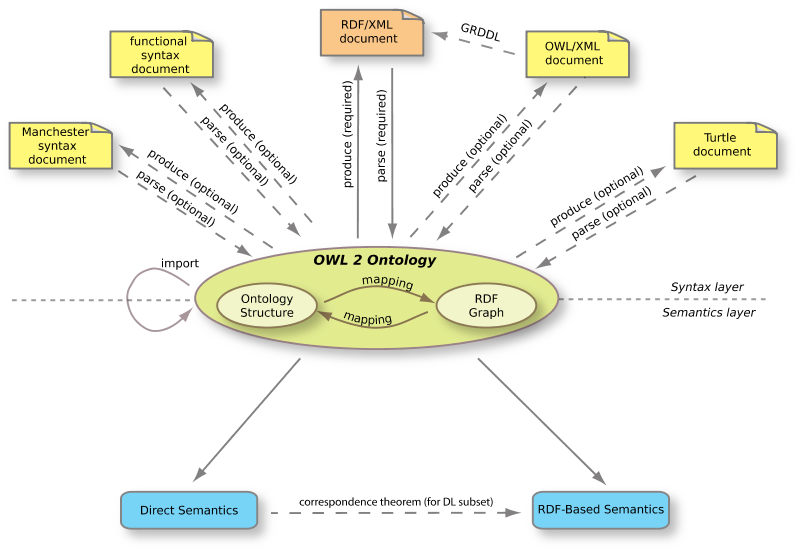
\includegraphics[width=1\textwidth]{owl_2_structure}
	\caption{Struktur OWL 2.0}
	\label{fig:owl_2_structure}
\end{figure}

Masing-masing format sintak memiliki kelebihan dan kekurangan. Format RDF/XML memiliki dukungan yang paling baik, hanya saja kurang intuitif jika dibandingkan dengan Turtle, Functional maupun Manchester, sedangkan Turtle Functional dan Manchester tidak memiliki dukungan \emph{tool} yang baik.
\begin{itemize}
	\item contoh sintak RDF/XML \\
	\begin{lstlisting}
		<SubClassOf>
			<Class IRI="Woman"/>
			<Class IRI="Person"/>
		</SubClassOf>
	\end{lstlisting}

	\item contoh sintak functional \\
	\begin{lstlisting}
		SubClassOf( :Woman :Person )
	\end{lstlisting}
	
	\item contoh sintak manchester
	\begin{lstlisting}
		Class: Woman
			SubClassOf: Person
	\end{lstlisting}

	\item contoh sintak turtle
		\begin{lstlisting}
			:Woman rdfs:subClassOf :Person .
		\end{lstlisting}
\end{itemize}

\subsection{Profil OWL 2}
Seperti yang telah dijelaskan sebelumnya bahwa OWL 1 memiliki tiga sub-bahasa, namun dalam praktiknya ketiga sub-bahasa tersebut ternyata belum cukup untuk memenuhi kebutuhan yang ada. \citet{patel} mengungkapkan beberapa permasalahan dalam \emph{real world application} yang diadapi para pengembang.

Berdasarkan fakta tersebut, maka OWL 2 membagi sub-bahasa kedalam tiga bagian yaitu:
\begin{itemize}
	\item OWL 2 EL
	\item OWL 2 QL
	\item OWL 2 RL
\end{itemize}

Masing-masing profil dibatasi oleh batasan sintaks \emph{(syntactic restriction)}. Perlu diketahui bahwa sub-bahasa OWL 2 ini berdasarkan pada OWL-DL, sehingga semua ekspresi yang diyatakan valid pada OWL 2 EL misalnya, secara otomatis akan valid juga untuk OWL-DL. Gambar \ref{fig:owl_2_profile} menunjukkan diagram venn relasi antar sub-bahasa pada OWL 2.

\begin{figure}[h]
	\centering
	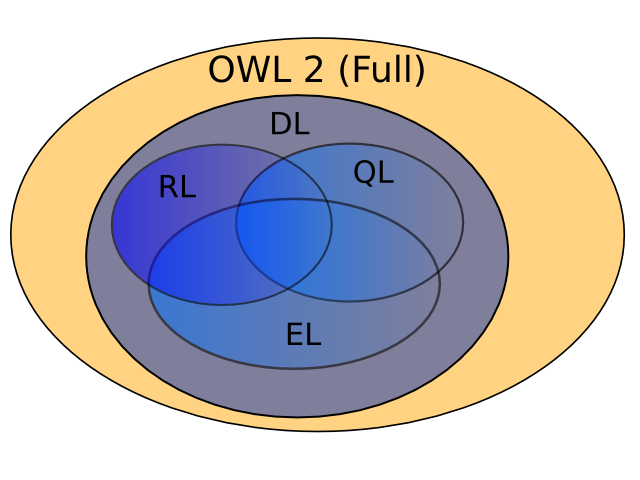
\includegraphics[scale=0.4]{owl_2_profile}
	\caption{Diagram venn profil OWL 2}
	\label{fig:owl_2_profile}
\end{figure}